\newacronym{va}{VA}{Visual Analytics}
\newacronym{ml}{ML}{Machine Learning}
\newacronym{hci}{HCI}{Human-Computer Interaction}
\newacronym{ux}{UX}{User Experience}
\newacronym{ui}{UI}{User Interface}
\newacronym{ir}{IR}{Information Retrieval}
\newacronym{infovis}{InfoVis}{Information Visualization}
\newacronym{cvast}{CVAST}{Centre for Visual Analytics Science and Technology}

\newglossaryentry{datascience}
{
  name={data science},
  description={concerns itself with gaining insights from data scientifically}
}
\newglossaryentry{datawrangling}
{
  name={data wrangling},
  description={consists of techniques being applied to transform data}
}
\newglossaryentry{datamunging}
{
  name={data munging},
  description={is a synonym for \gls{datawrangling}}
}
\newglossaryentry{datamining}
{
  name={data mining},
  description={consists of techniques being applied, mainly , for \gls{ml}}
}


\section{Motivation}

Applied work within \gls{datascience}, and more specifically \textbf{\gls{va}}, \emph{``the science of
analytical reasoning facilitated by interactive visual interfaces''}~\cite{Thomas2005} (p. 4), can be seen to roughly consist of three main basic building blocks~\cite{Web:DataScience}:
\begin{enumerate}
  \item \textbf{\Gls{datawrangling}} a.k.a. \textbf{\glslink{datamunging}{munging}}
  \item Statistics\index{statistics} \& \Gls{ml}
  \item Visualization \& analysis\index{analysis} itself
\end{enumerate}

While the second and last mentioned fields are constantly evolving related tools and techniques, the first one is comparatively still lacking in terms of high-level support.
This is when it comes down to actually wrangle\index{wrangle} usually messy real-world data into a format prepping it useful for analysis\index{analysis}.

To this day, it mostly means fiddling around with the data manually, applying hand-crafted transformation\index{transformation} scripts.
This is a tedious task and discourages analyzing data altogether, especially if the ones intending to work with the data are technically unversed (for instance, journalists or business analysts).

However, combining contemporary knowledge and technology from the domains of \emph{\gls{hci}}~\cite{Cooper2004} \& \emph{\gls{ux}}~\cite{Norman2002} as well as \emph{\gls{ir}}~\cite{Manning2008}, \emph{\gls{datamining}} / \emph{\Gls{ml}}~\cite{Witten2011}, and \emph{\gls{infovis}}~\cite{Tufte2001}~\cite{Card1999}, could yield substantial improvements here.

Namely, making \gls{datawrangling} accessible to a wider audience, mainly by providing interactive analytical visualizations allowing for easy data transformations\index{transformation} and giving immediate visual feedback.

In this thesis we are investigating the field of \gls{datawrangling}, plus, designing\index{design}, and prototypically\index{prototype} implementing a \gls{va} approach\index{approach} to support the tasks involved.
That is, iteratively creating a software prototype\index{prototype} which enables users to wrangle\index{wrangle} data suitable for analysis\index{analysis} in an intuitive, interactive, and visual way.

\Gls{va} and \gls{infovis} enable uncovering the non-obvious by using interactive visualizations.
Consequently, this approach is especially useful when applied to complex tasks where clear overview and structuring is necessary in order to achieve effective results efficiently.
That is also why employing related techniques can generally be expected to be more successful for the outlined use case than fully automated ones.
Hence, an ideal solution would probably be a blend of automated suggestions, augmenting an interactive interface driven by visualizations.

Additionally, the to-be-developed prototype\index{prototype} shall, in particular, make it convenient to work on time-oriented\index{time-oriented} datasets. Time itself and time-oriented\index{time-oriented} data, specifically, possess distinct characteristics (for instance, regarding scale, scope, structure, viewpoint, and granularity) that make it worthwhile to dedicatedly treat it as a separate data type, as suggested by Aigner et al.~\cite{Aigner2011}.
This is why time-oriented\index{time-oriented} data demands for special \gls{datawrangling} solutions which have not been adequately tackled yet.


\section{Problem Statement}

The main research question in the context of this work is:

\textbf{\emph{How can we support \gls{datawrangling} with \gls{va} techniques?}}
\\\\
More particular, we are to tackle the following subquestions:

\begin{itemize}
  \item \emph{Which data transformations\index{transformation} are best supported by analytical methods and for which transformations\index{transformation} is visual support beneficial?}
  \item \emph{How do concrete \gls{datawrangling} workflow processes look like and how can these processes be supported by \gls{va} methods?}
  \item \emph{What \gls{datawrangling} tasks need to be tackled in particular when dealing with time-oriented\index{time-oriented} data and how can we support them with \gls{va} methods?}
\end{itemize}

The emphasis of this thesis is put on evaluating the feasibility of corresponding concepts via iterative design\index{design}, implementation, and evaluation of a software prototype\index{prototype}.


\section{Aim of the Work}

Results to be achieved are:

\begin{itemize}
  \item Design\index{design} and implementation of a research prototype\index{prototype}
  \item Evaluation of the prototype to answer research questions
  \item Detailed documentation of these
\end{itemize}

At the end of the project, it should be known whether developing such a \textbf{prototype}\index{prototype} supporting these tasks is feasible and if so, how in detail.
As mentioned above, the approach\index{approach} shall combine concepts from \gls{hci} \& \gls{ux} with ones from \gls{ir}, \gls{ml}, and \gls{va}.
Special focus will be laid on crafting the \textbf{\gls{ui}} and an underlying \textbf{analytical inference engine}, interactively providing the user with respective data quality and potential issue suggestions visually. Furthermore, \textbf{direct manipulation} of data should be easy.
Plus, transformations\index{transformation} shall, generally, be easily applicable to \textbf{batches of data} by making use of bulk operations, while again being visual-interactively supported.
A central challenge is making this all work in the context of \textbf{time-oriented\index{time-oriented} data}.

Answers to the stated research questions are intended to be given by designing\index{design}, implementing, and evaluating a research prototype\index{prototype} which provides \gls{va} techniques to improve and support \gls{datawrangling} tasks.


\section{Methodological Approach}

In order to answer our research questions we follow the nested model by Munzner~\cite{Munzner2009}. In particular we include the following steps:

\begin{enumerate}
  \item \textbf{State of the art review}: giving an overview of the topic, spanning from scientific foundation to various approaches\index{approach}, and serving as first input to our approach\index{approach}.
  \item \textbf{Requirements analysis\index{analysis}}: determining which features to implement, directed to answering why, what, and how.
  \item \textbf{Design\index{design} of interactive visualizations}: subsequent iterative design\index{design} process, making use of state-of-the-art tools.
  \item \textbf{Iterative prototypical\index{prototype} implementation}: following an agile approach\index{approach} until satisfying results are achieved.
  \item \textbf{Qualitative evaluation of results}: for validating fulfillment of goals and, consequently, leading to answering our research questions.
\end{enumerate}

In the context of this work, we also consider the \emph{data--users--tasks} triangle for \gls{va}.
This triangle can be seen in Figure~\ref{fig:cvast-triangle} and is introduced in \cite{Miksch2014}.
It is particularly useful for initial requirements analysis\index{analysis} of a visualization project.
Consequently, we apply it as a starting point.
Its basic notion is to think of a product for \gls{va} within the three dimensions of data, users, and tasks separately, first, and then in interplay.
The latter, thus, defines effectiveness, expressiveness, and appropriateness of the to-be-chosen interactive \gls{va} methods, as visualized in the diagram.

\begin{figure}[h]
  \centering
  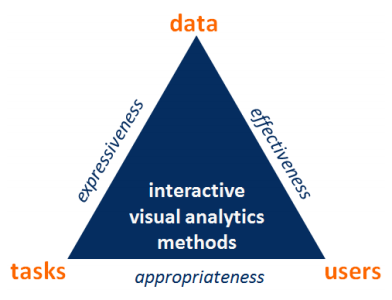
\includegraphics[width=0.725\textwidth]{figures/introduction/cvast-triangle}
  \caption{The \emph{data--users--tasks} triangle as presented in \cite{Miksch2014}.}
  \label{fig:cvast-triangle}
\end{figure}

All steps are accurately documented, emphasizing findings of the evaluation and lessons learned.
The thesis covers all aspects and results of the design\index{design}, development, and evaluation of the prototype\index{prototype}, from mockups and architectural\index{architecture} diagrams to test results.


\section{Structure of the Work}

The thesis is structured as follows:

\begin{enumerate}
  \item An \textbf{introduction} to the topic and thesis itself: this presents the motivation, problem statement, and methodological approach\index{approach}.
  \item A \textbf{state of the art} review: this is laying out the scientific foundation regarding our topic and showing various approaches\index{approach}. The latter are, thus, analyzed and compared. It is closed by a crossover to the requirements analysis\index{analysis} for our approach\index{approach}, fueled with preceding input.
  \item A \textbf{design\index{design} and implementation} chapter: this is describing, explaining, and documenting all connected steps thoroughly. The design\index{design} section consists of creating personas, wireframing with mockups, and consequently deriving our requirements. The implementation section walks through the developed prototype\index{prototype}, looking at it from varied angles, and presents its qualitative evaluation.
  \item A concluding section with \textbf{critical reflection} of the achieved work: this includes comparing with related work, discussing open issues, and answering our research questions. It is also concerning the requirements we have previously derived.
  \item Finally, closing the thesis with a \textbf{summary and future work} section: this is just briefly summing up our work and offering an outlook.
  \item At the end, there is an \textbf{appendix}: this contains a detailed presentation of the software design\index{design} and architecture\index{architecture} of our prototype\index{prototype} as well as scientific background, plus further implementation details.
\end{enumerate}
